\documentclass[aspectratio=169]{beamer}
\usetheme{metropolis}           % Use metropolis theme

\usepackage{braket}
\usepackage{amsmath}
\usepackage{cancel}
\usepackage{color}

\setlength{\parindent}{0em}

\newcommand{\backupbegin}{
   \newcounter{finalframe}
   \setcounter{finalframe}{\value{framenumber}}
}
\newcommand{\backupend}{
   \setcounter{framenumber}{\value{finalframe}}
}

\title{
  Analysis of three-body effects \\
  in the in-medium similarity renormalization group
}
\date{October 21, 2020}
\author{Matthias Heinz}
\institute{Institut f\"ur Kernphysik, TU Darmstadt}
\begin{document}

% TODO
\newcommand{\XXX}[1]{\textcolor{red}{#1}}

% Text shortcuts
\newcommand{\mscheme}{\texorpdfstring{$m$-scheme}{m-scheme}\xspace}
\newcommand{\abinitio}{\textit{ab initio}\xspace}

% Units
\newcommand{\mev}{\, \text{MeV}}
\newcommand{\invfm}{\, \text{fm}^{-1}}

% Second quant
\newcommand{\crea}[1]{\ensuremath{a_{#1}^{\dagger}}}
\newcommand{\annih}[1]{\ensuremath{a_{#1}}}
\newcommand{\qpcrea}[1]{\ensuremath{b_{#1}^{\dagger}}}
\newcommand{\qpannih}[1]{\ensuremath{b_{#1}}}

% Commutators
\newcommand{\comm}[2]{\ensuremath{[#1, #2]}}
\newcommand{\anticomm}[2]{\ensuremath{\{#1, #2\}}}

% A-body operators
\newcommand*{\zerobodyop}[1]{\ensuremath{{#1}^{(0)}}}
\newcommand*{\onebodyop}[1]{\ensuremath{{#1}^{(1)}}}
\newcommand*{\twobodyop}[1]{\ensuremath{{#1}^{(2)}}}
\newcommand*{\threebodyop}[1]{\ensuremath{{#1}^{(3)}}}
\newcommand*{\abodyop}[1]{\ensuremath{{#1}^{(A)}}}

% Normal ordering
\newcommand{\nogen}[1]{\ensuremath{\text{N}\left[#1\right]}}
\newcommand{\novac}[1]{\ensuremath{\text{N}_{0}\left[#1\right]}}
\newcommand{\noref}[1]{\ensuremath{\text{N}_{\Phi}\left[#1\right]}}

% Normal ordered operators
\newcommand*{\hnozero}{\zerobodyop{\bar{H}}}
\newcommand*{\hnoone}{\onebodyop{\bar{H}}}
\newcommand*{\hnotwo}{\twobodyop{\bar{H}}}
\newcommand*{\hnothree}{\threebodyop{\bar{H}}}


% Ref state
\newcommand{\refgnd}{\ensuremath{\ket{\Phi}}}
\newcommand{\refhp}[2]{\ensuremath{\ket{\Phi_{#1}^{#2}}}}

% IM_SRG generators
\newcommand*{\genone}{\eta^{(1)}}
\newcommand*{\gentwo}{\eta^{(2)}}
\newcommand*{\genthree}{\eta^{(3)}}

% m-scheme basis
\newcommand*{\emax}{e_{\text{max}}}

\maketitle

% \section{Motivation}

\begin{frame}{\textit{Ab initio} nuclear structure}
  \vskip-1.5em
  \begin{columns}[t]
    \begin{column}{0.5\textwidth}
      \vskip1.5em
      \textit{Ab initio} approach:
      \begin{enumerate}
        \item Determine nuclear interactions
        \item Solve many-body problem
        \item (1) \& (2) should be systematically improvable
      \end{enumerate}
      Benefits:
      \begin{itemize}
        \item Physics insights
        \item Predictive power
        \item Quantify uncertainties
      \end{itemize}
    \end{column}
    \begin{column}{0.50\textwidth}
      \begin{center}
        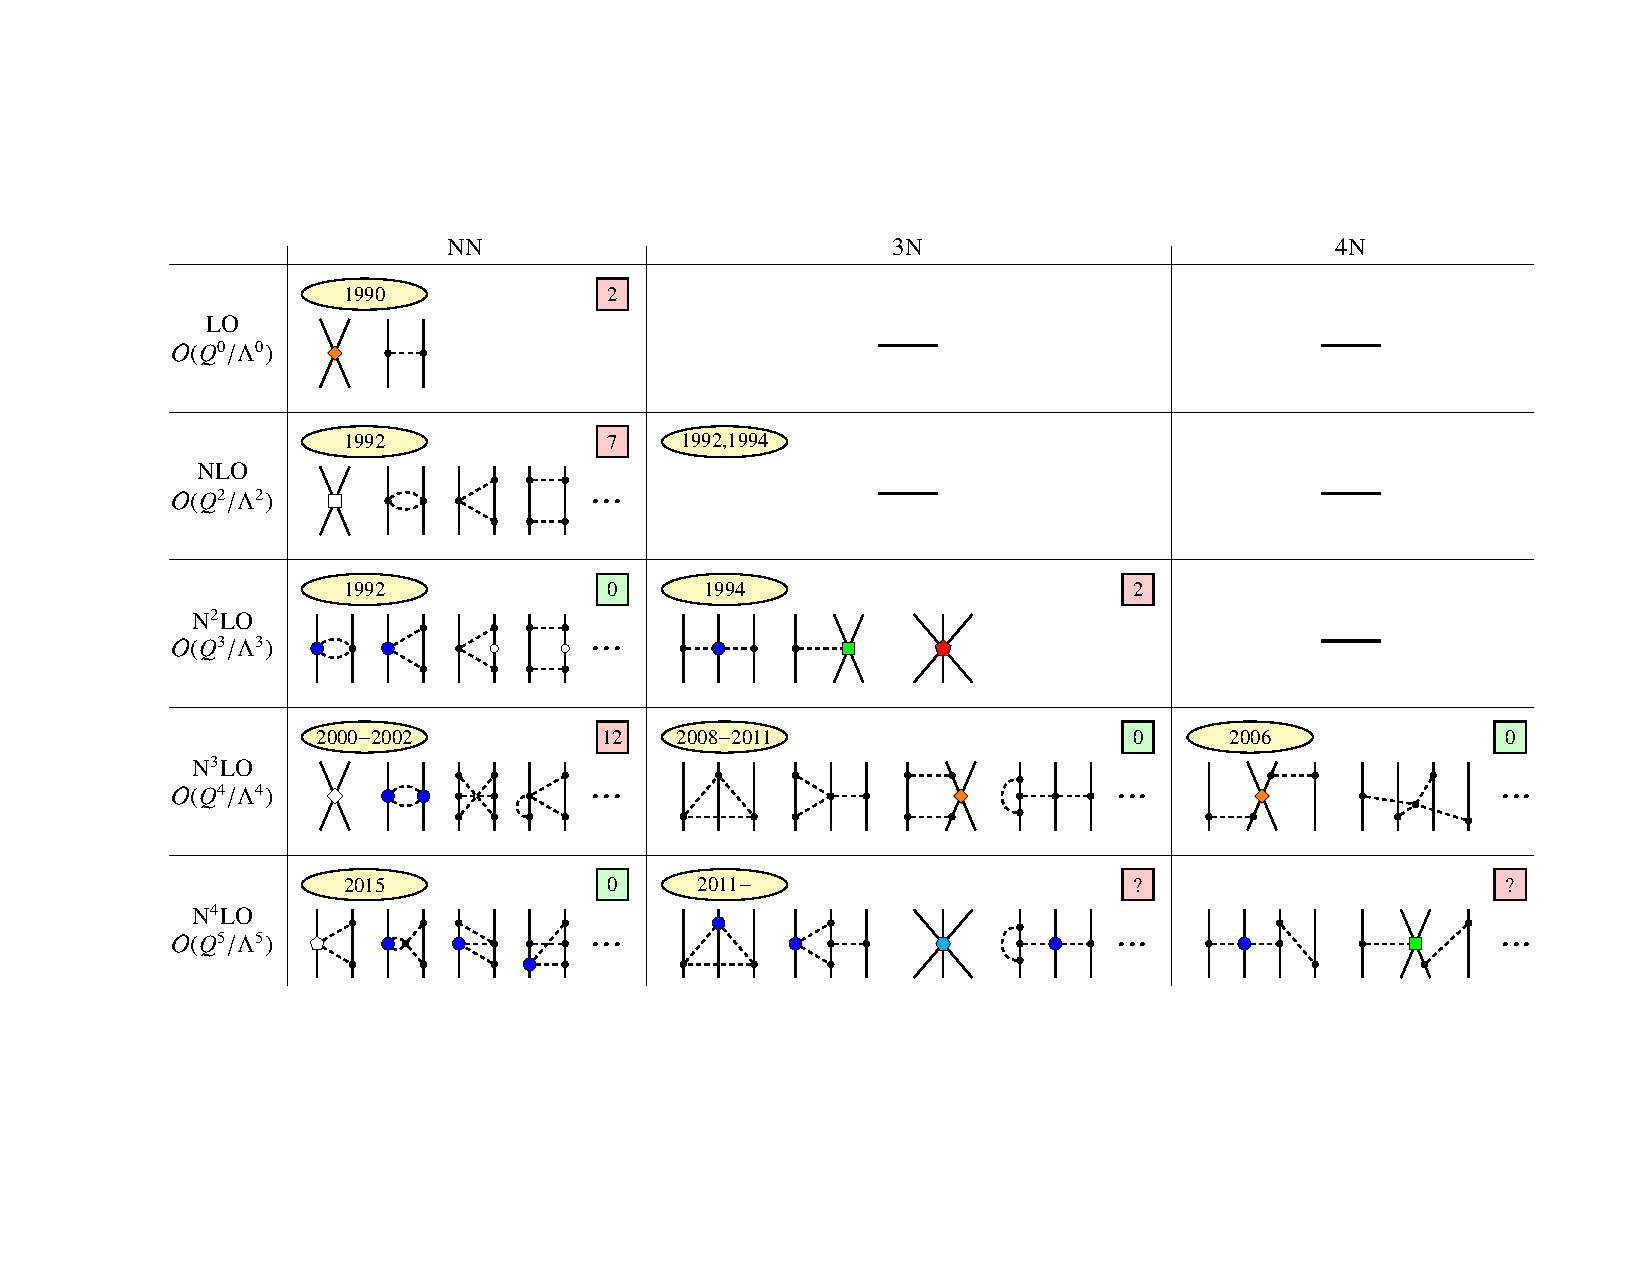
\includegraphics[width=0.9\textwidth]{thesis/talk/images/external/table_norefs.pdf} \\\vskip0.8em
        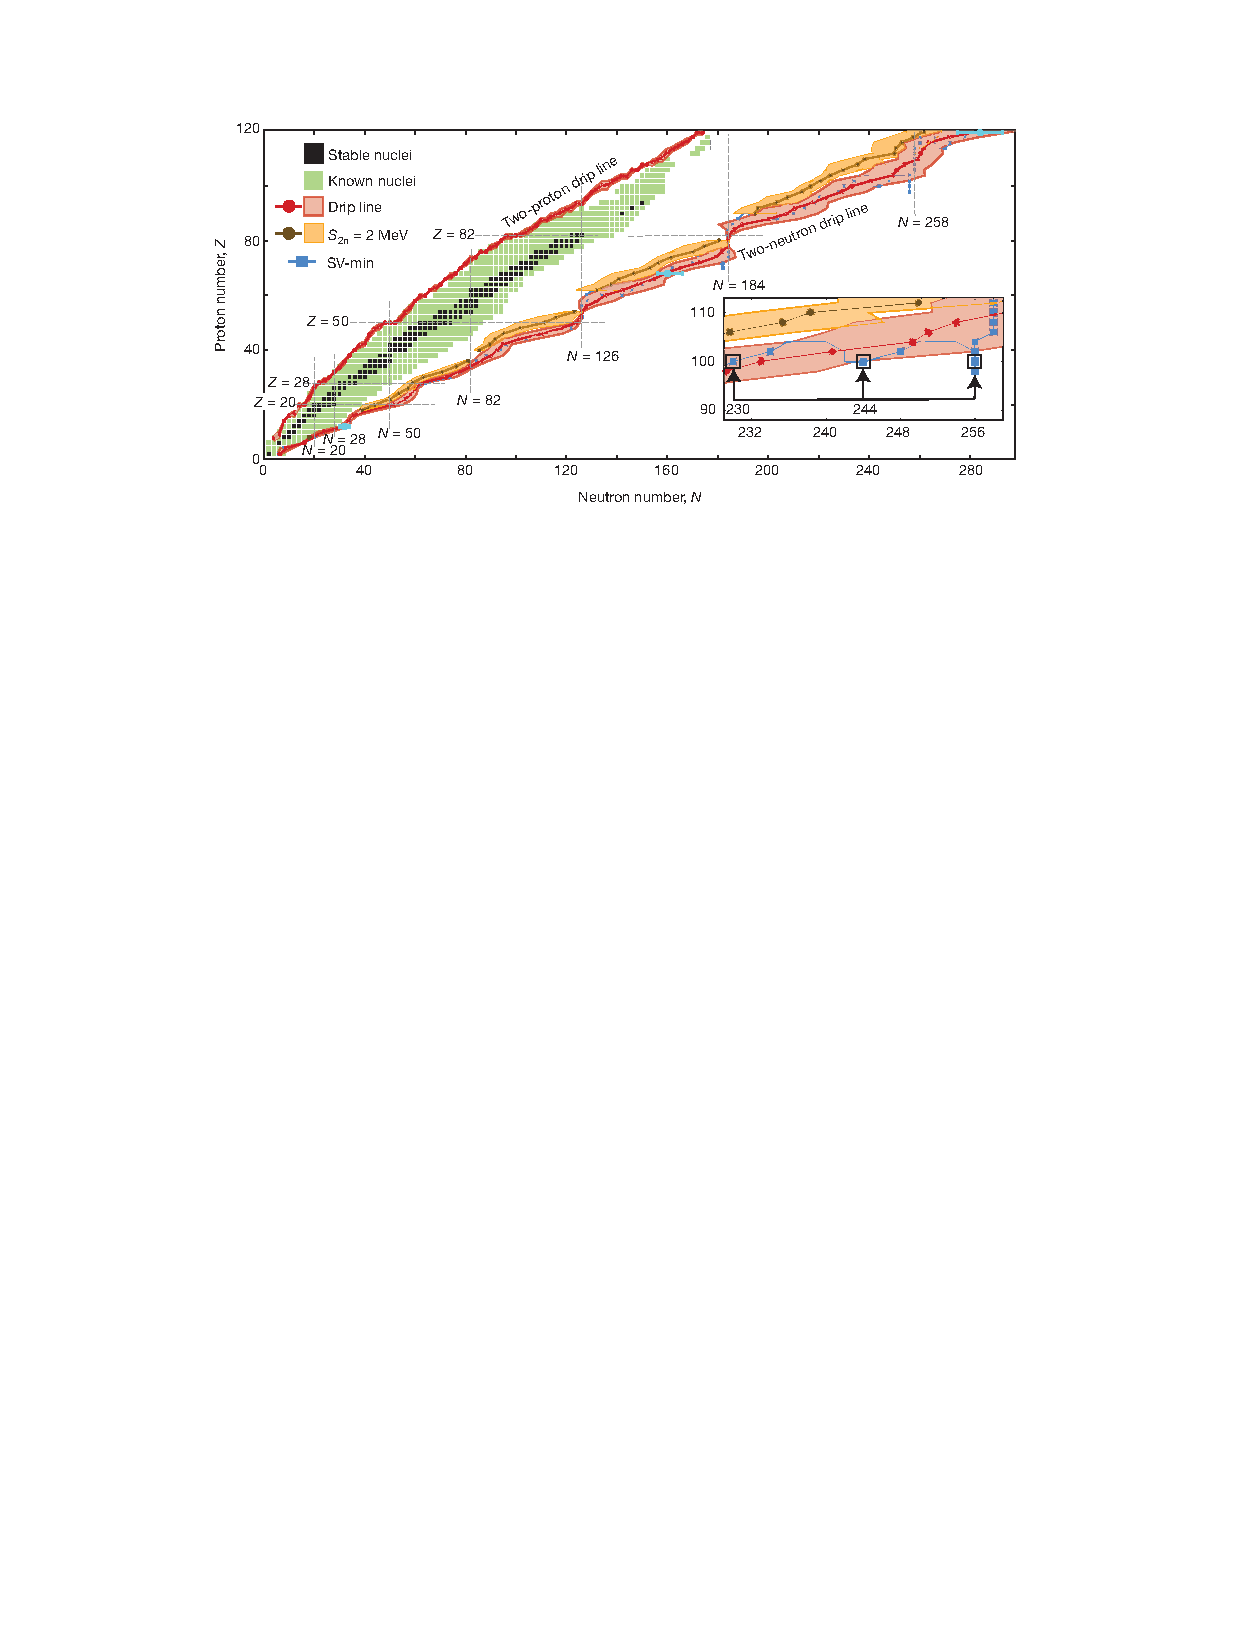
\includegraphics[width=0.9\textwidth]{thesis/talk/images/external/nuclear_landscape_embedded.pdf} \\
        {\tiny Top: Hebeler, 2020, Bottom: Erler \textit{et al.}, Nature \textbf{486}, 2012}
      \end{center}
    \end{column}
  \end{columns}
\end{frame}

\begin{frame}{Recent \textit{ab initio} progress}
  \begin{columns}[t]
    \begin{column}{0.4\textwidth}
      \begin{itemize}
        \item 2010: mostly results in range of exact methods (NCSM, QMC)
        \item 2010-2015: many-body expansion methods able to target (near) closed-shell nuclei
        \item 2015-2020: full \textit{ab initio} description of mid-mass open- and closed-shell systems
      \end{itemize}

    \end{column}
    \begin{column}{0.60\textwidth}
      \begin{center}
        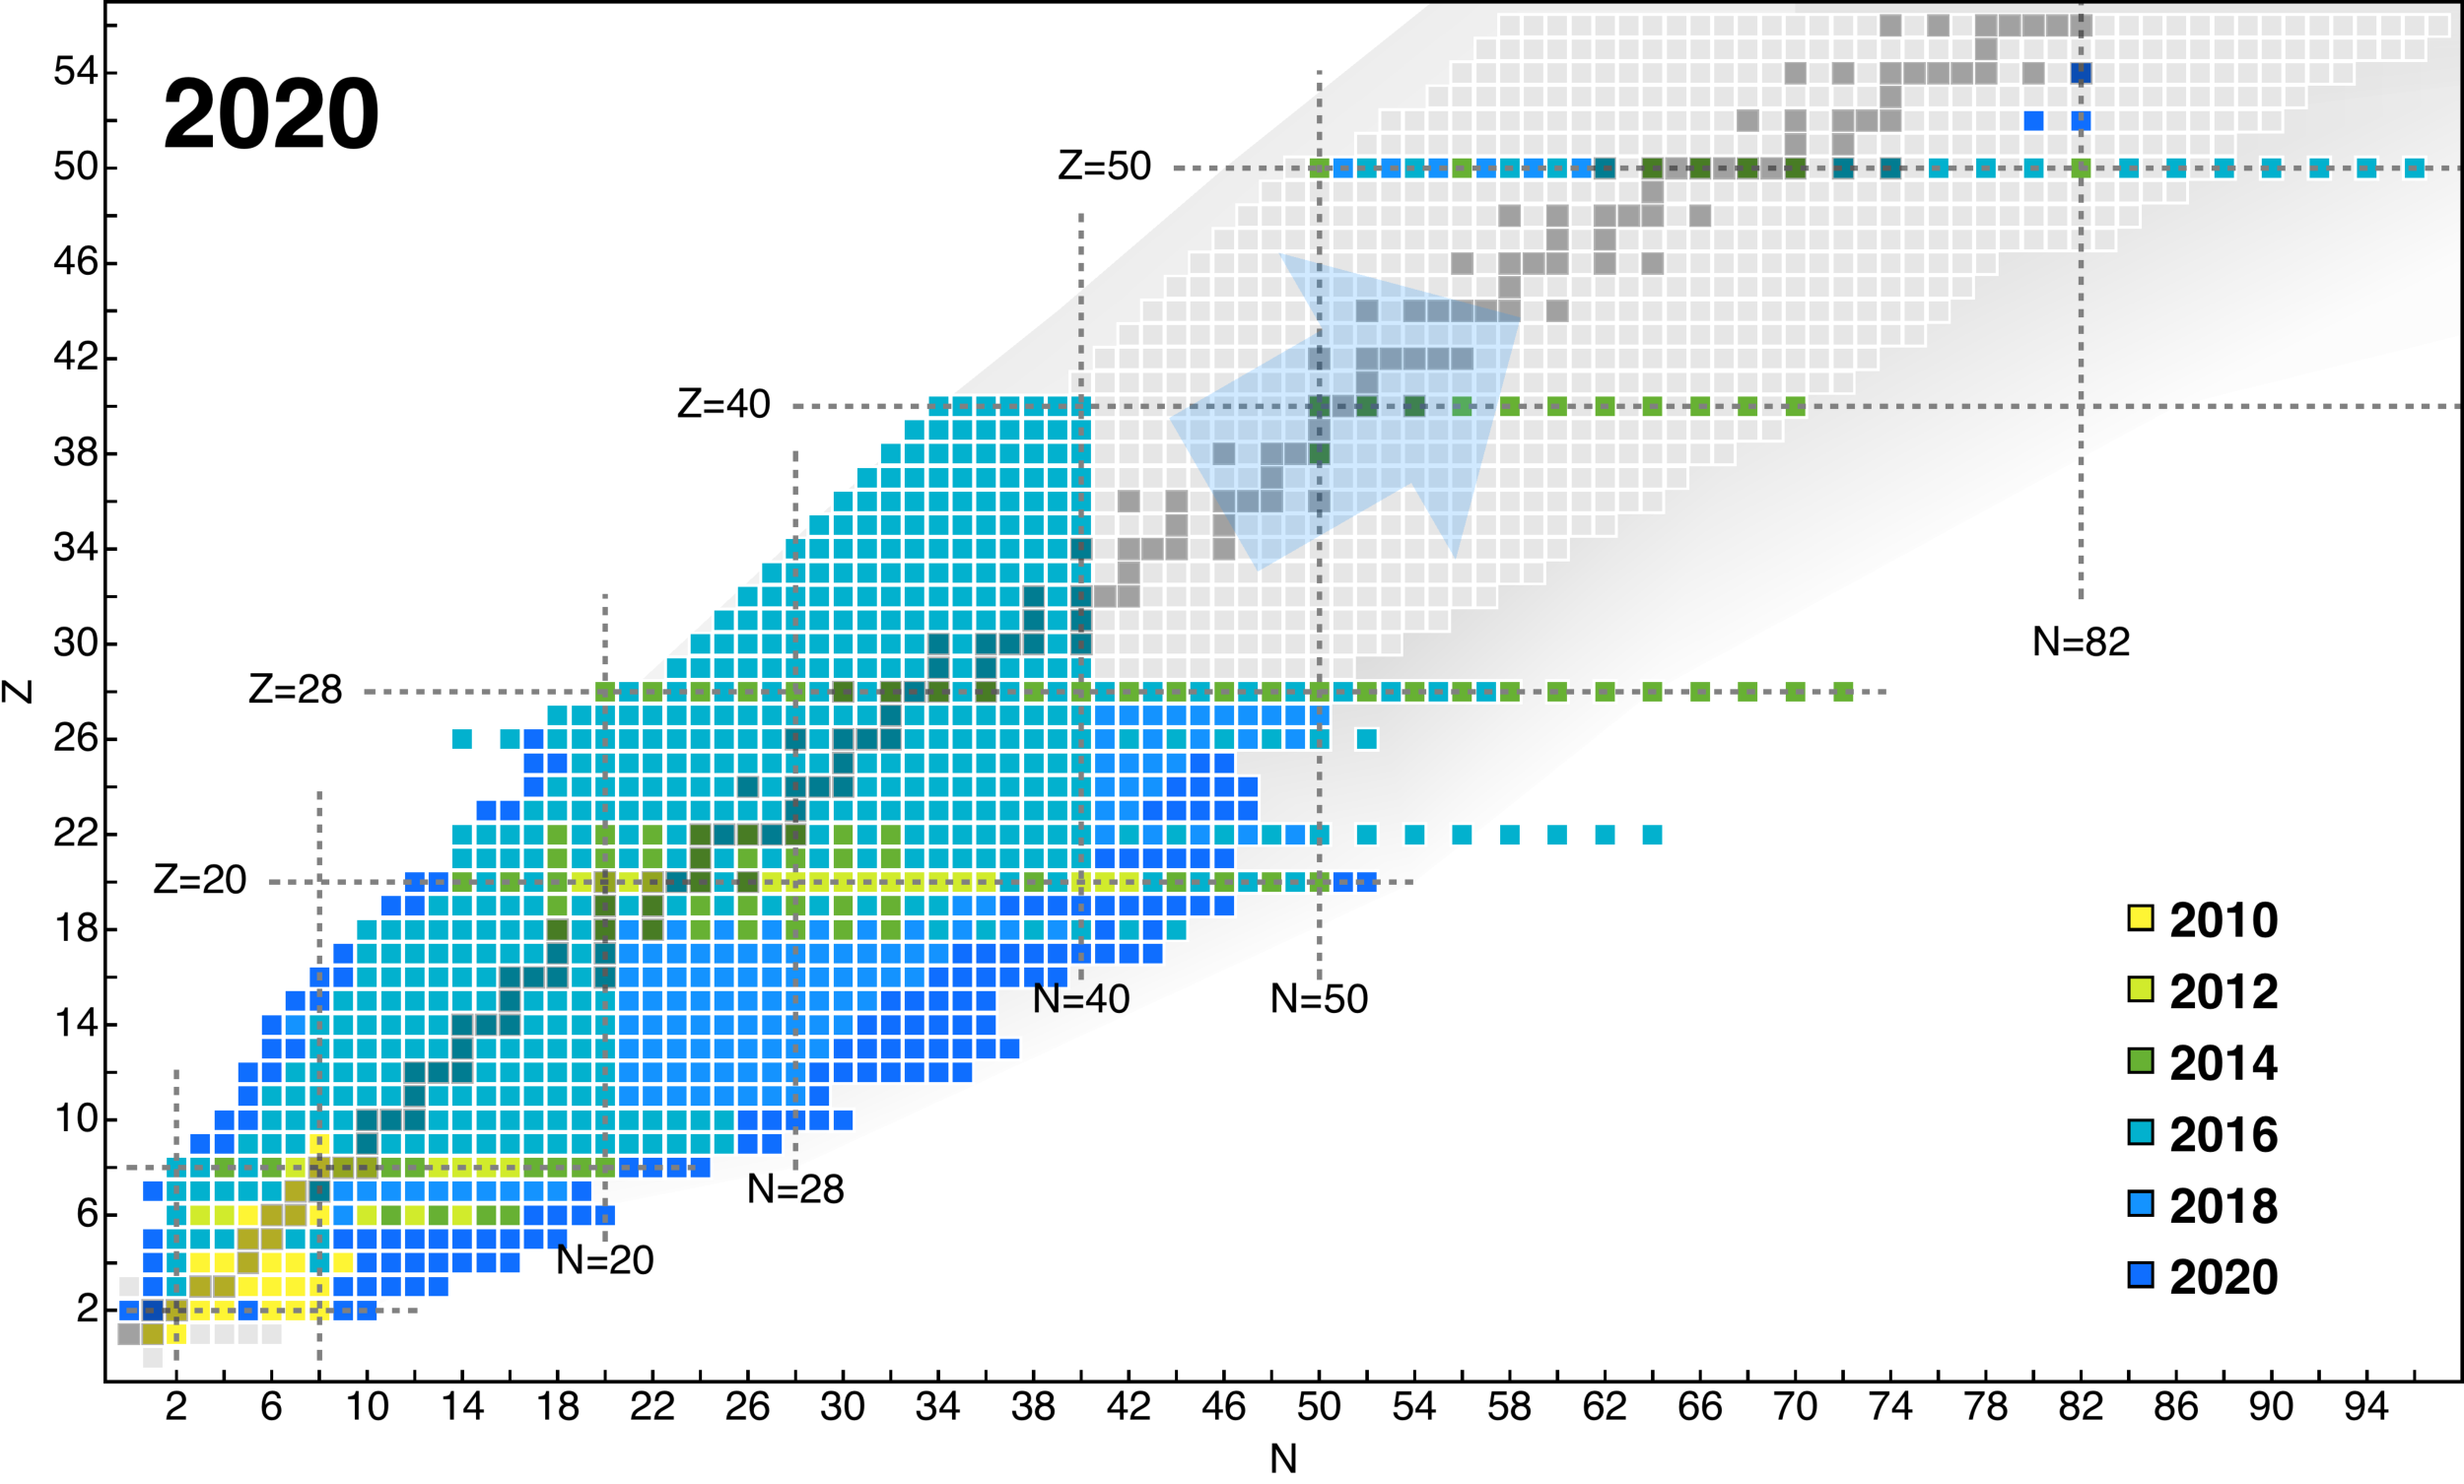
\includegraphics[width=\textwidth]{thesis/talk/images/external/ab_initio_progress.pdf} \\
        {\tiny Hergert, Front.~Phys.~\textbf{8}, 2020}
      \end{center}
    \end{column}
  \end{columns}
\end{frame}

\begin{frame}{Essence of many-body expansion methods}
  \vskip1.0em
  \begin{columns}[t]
    \begin{column}{0.7\textwidth}
      Examples: CI, MBPT, CC, SCGF, IMSRG
      \begin{equation*}
        \ket{\Psi} \approx \ket{\Phi} \visible<2->{+ \sum_{ia} c_{i}^{a} \ket{\Phi_{i}^{a}} +  \sum_{ijab} c_{ij}^{ab} \ket{\Phi_{ij}^{ab}} + \ldots}
      \end{equation*}
      % \only<2->{\begin{equation*}
      %     \ket{\Psi} \approx \ket{\Phi} +  \sum_{ia} c_{i}^{a} \ket{\Phi_{i}^{a}} +  \sum_{ijab} c_{ij}^{ab} \ket{\Phi_{ij}^{ab}} + \ldots
      %   \end{equation*}}
      \visible<3->{Normal order w.r.t.~$\ket{\Phi}$ to pull out $E=\hnozero=\braket{\Phi|H|\Phi}$:
        \begin{equation*}
          \onebodyop{H} + \twobodyop{H} + \threebodyop{H}
          \rightarrow \hnozero + \hnoone + \hnotwo + \hnothree
        \end{equation*}}

      \vskip-1.75em
      \visible<4->{Systematically construct corrections to $\ket{\Phi}$\\
        and corrections to observables (ex.~MBPT)}


    \end{column}
    \begin{column}{0.30\textwidth}
      \begin{center}
        \begin{overprint}
          \onslide<1>\centering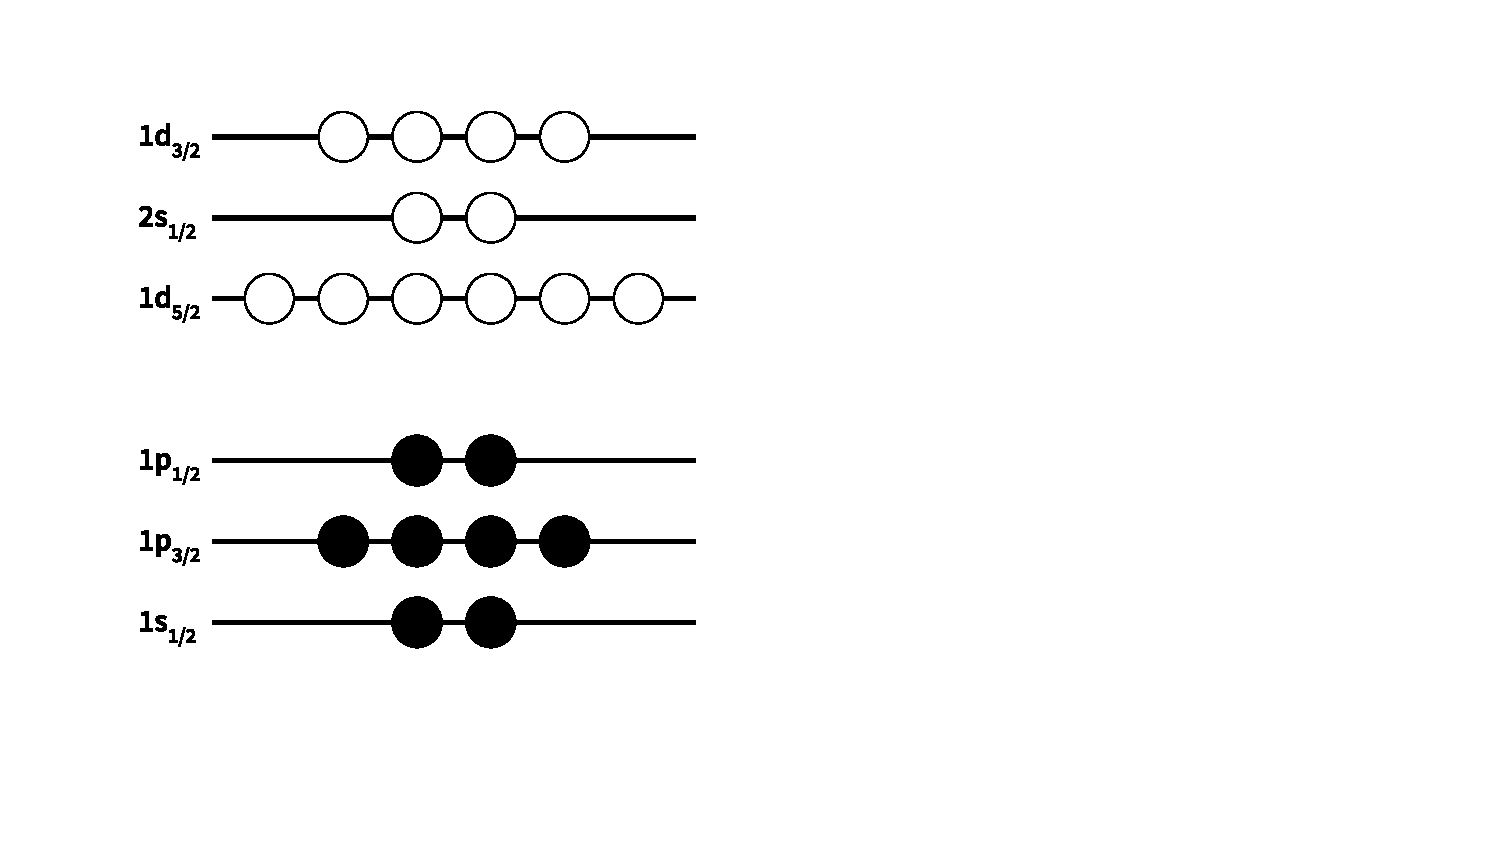
\includegraphics[trim=2cm 2.5cm 13cm 1.5cm, clip, width=0.95\textwidth]{thesis/talk/images/o16_reference_state.pdf}
          \onslide<2->\centering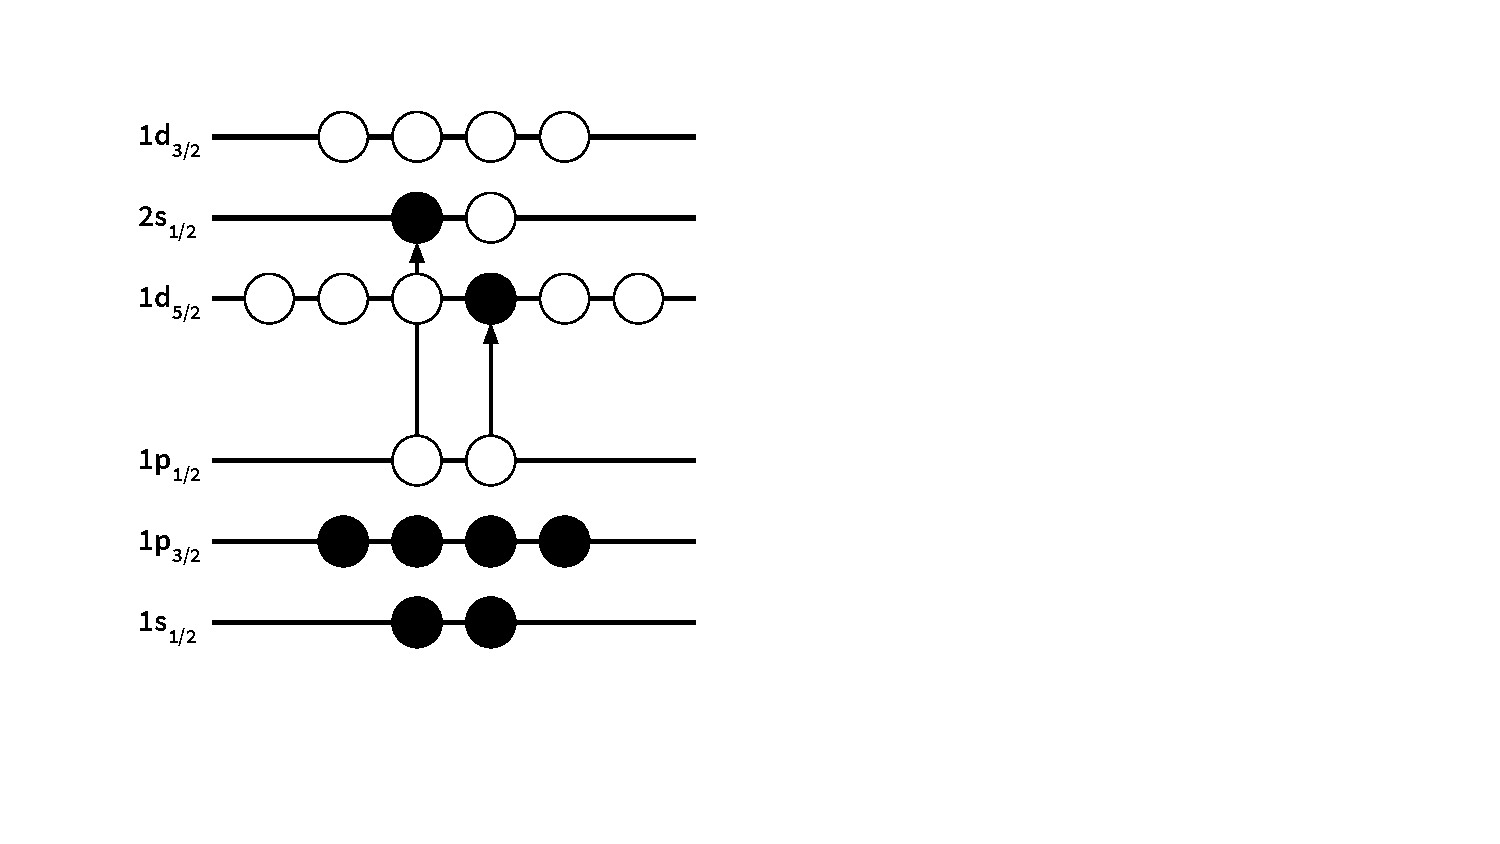
\includegraphics[trim=2cm 2.5cm 13cm 1.5cm, clip, width=0.95\textwidth]{thesis/talk/images/o16_2p2h_state.pdf}
          % \onslide<4>\centering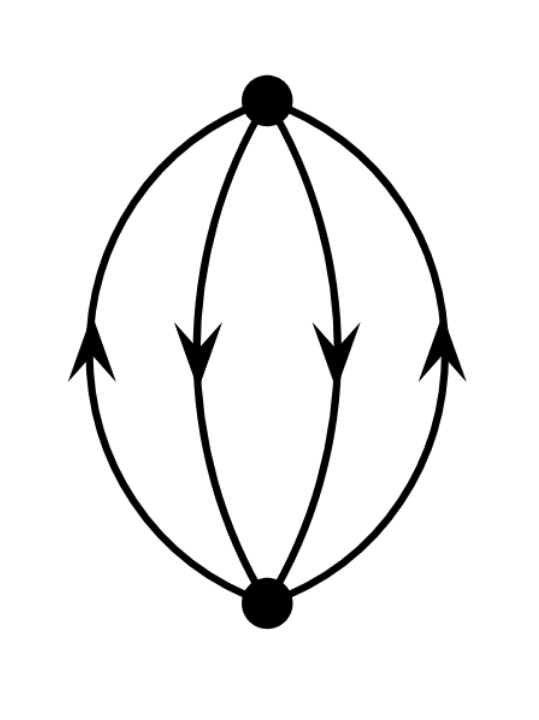
\includegraphics[trim=0cm 2.5cm 0cm 2.5cm, clip, width=0.85\textwidth]{thesis/talk/images/external/mp2.png}
        \end{overprint}
        \only<1>{$\phantom{\ket{\Phi_{ij}^{ab}}}\ket{\Phi}\phantom{\ket{\Phi_{ij}^{ab}}}$}
        \only<2->{$\phantom{\ket{\Phi_{ij}^{ab}}}\ket{\Phi_{ij}^{ab}}\phantom{\ket{\Phi_{ij}^{ab}}}$}
      \end{center}
    \end{column}
  \end{columns}
  \begin{center}
    \visible<5->{IMSRG formalism gives rise to IMSRG(2) and IMSRG(3) truncations}
  \end{center}
\end{frame}

\begin{frame}{IMSRG(3) in the many-body context}
  \vskip0.5em
  \begin{columns}[t]
    \begin{column}{0.40\textwidth}
      Many-body expansion is \\ ``under control''

      \vskip0.5em
      Why go to IMSRG(3)?
      \begin{itemize}
        \item Confirm many-body expansion behavior
        \item Higher precision in light and medium-mass nuclei
        \item UQ for many-body expansion
        \item Approximate IMSRG(3) for heavy nuclei
        \item Study behavior for other observables
      \end{itemize}
    \end{column}
    \begin{column}{0.60\textwidth}
      \begin{center}
        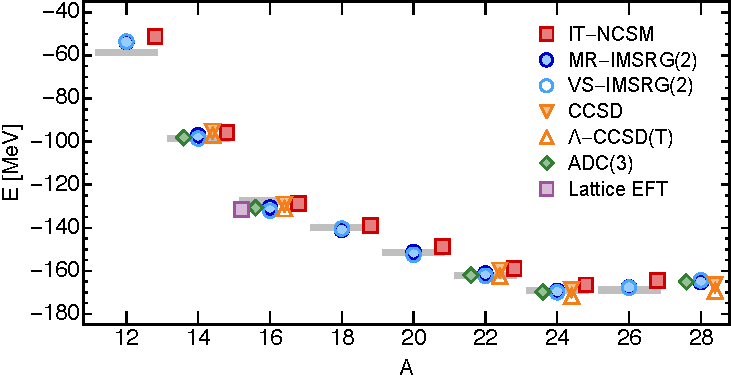
\includegraphics[width=\textwidth]{thesis/talk/images/external/ab_initio_comparison_oxygen.pdf} \\
        {\tiny Hergert, Front.~Phys.~\textbf{8}, 2020}
      \end{center}
    \end{column}
  \end{columns}
\end{frame}

\begin{frame}{Similarity renormalization group {\normalfont {\tiny Bogner, Furnstahl, Perry, PRC \textbf{75}, 2007}}}
  \begin{center}
    \vskip-0.5em
    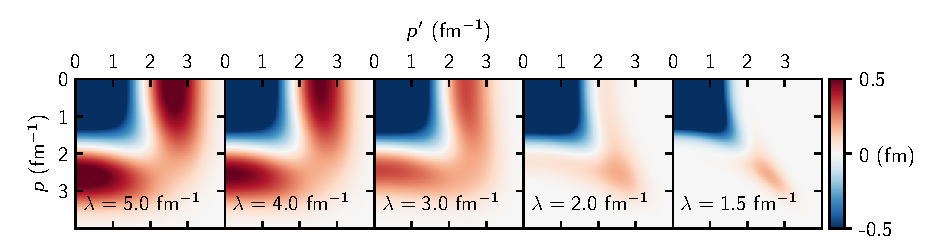
\includegraphics[width=0.8\textwidth]{thesis/talk/images/vnn_srg_emn500_n3lo.pdf}
  \end{center}
  \vskip-1.5em
  Continuous unitary transformation:
  \begin{align*}
    H(s)             & = U(s) H(s = 0) U^{\dagger}(s)\,, &
    \frac{dH(s)}{ds} & = \comm{\eta(s)}{H(s)}
  \end{align*}
  The SRG evolution\ldots
  \begin{itemize}
    \item decouples low- and high-energy states,
    \item but induces many-body forces.
  \end{itemize}
\end{frame}

\begin{frame}{In-medium similarity renormalization group (IMSRG) {\normalfont {\tiny Tsukiyama, Bogner, Schwenk, PRL \textbf{106}, 2011}}}
  \begin{equation*}
    \frac{dH(s)}{ds} = \comm{\eta(s)}{H(s)}
  \end{equation*}

  ``In-medium'': normal order $H$, $\eta$, and $dH/ds$
  w.r.t.~$\ket{\Phi}$

  \pause
  IMSRG(\only<2-3>{2}\only<4>{3}):
  \begin{align*}
    H(s)    & \approx \hnozero(s) + \hnoone(s) + \hnotwo(s) \visible<4->{+\hnothree(s)} \\
    \eta(s) & \approx \genone(s) + \gentwo(s) \visible<4->{+ \genthree(s)}
  \end{align*}
  \begin{overprint}
    \onslide<3>
    NO2B approximation:
    \begin{itemize}
      \item Approximate treatment of initial three-body force
      \item $\hnotwo_{pqrs} = H^{(2)}_{pqrs} + \sum_{i} H^{(3)}_{pqirsi}$
    \end{itemize}
    \onslide<4>
    Normal ordering:
    \begin{itemize}
      \item Complete inclusion of initial normal-ordered Hamiltonian
      \item Approximate evolution of many-body forces (both IMSRG(2) and IMSRG(3))
    \end{itemize}
  \end{overprint}
\end{frame}

\begin{frame}{Decoupling in the IMSRG in closed-shell systems}

  \begin{columns}
    \begin{column}{0.42\textwidth}

      \begin{itemize}
        \item Decouple $\ket{\Phi}$ from its excitations
        \item $E(s\rightarrow \infty) = \braket{\Phi|H(s\rightarrow\infty)|\Phi}$
              is the energy of the targeted state
        \item Observe: MBPT corrections vanish
              for $s\rightarrow \infty$
      \end{itemize}
    \end{column}
    \begin{column}{0.58\textwidth}
      \setlength{\unitlength}{\columnwidth}
      \begin{center}
        \begin{picture}(1.0000,0.5500)
          \put(0.0350,0.0450){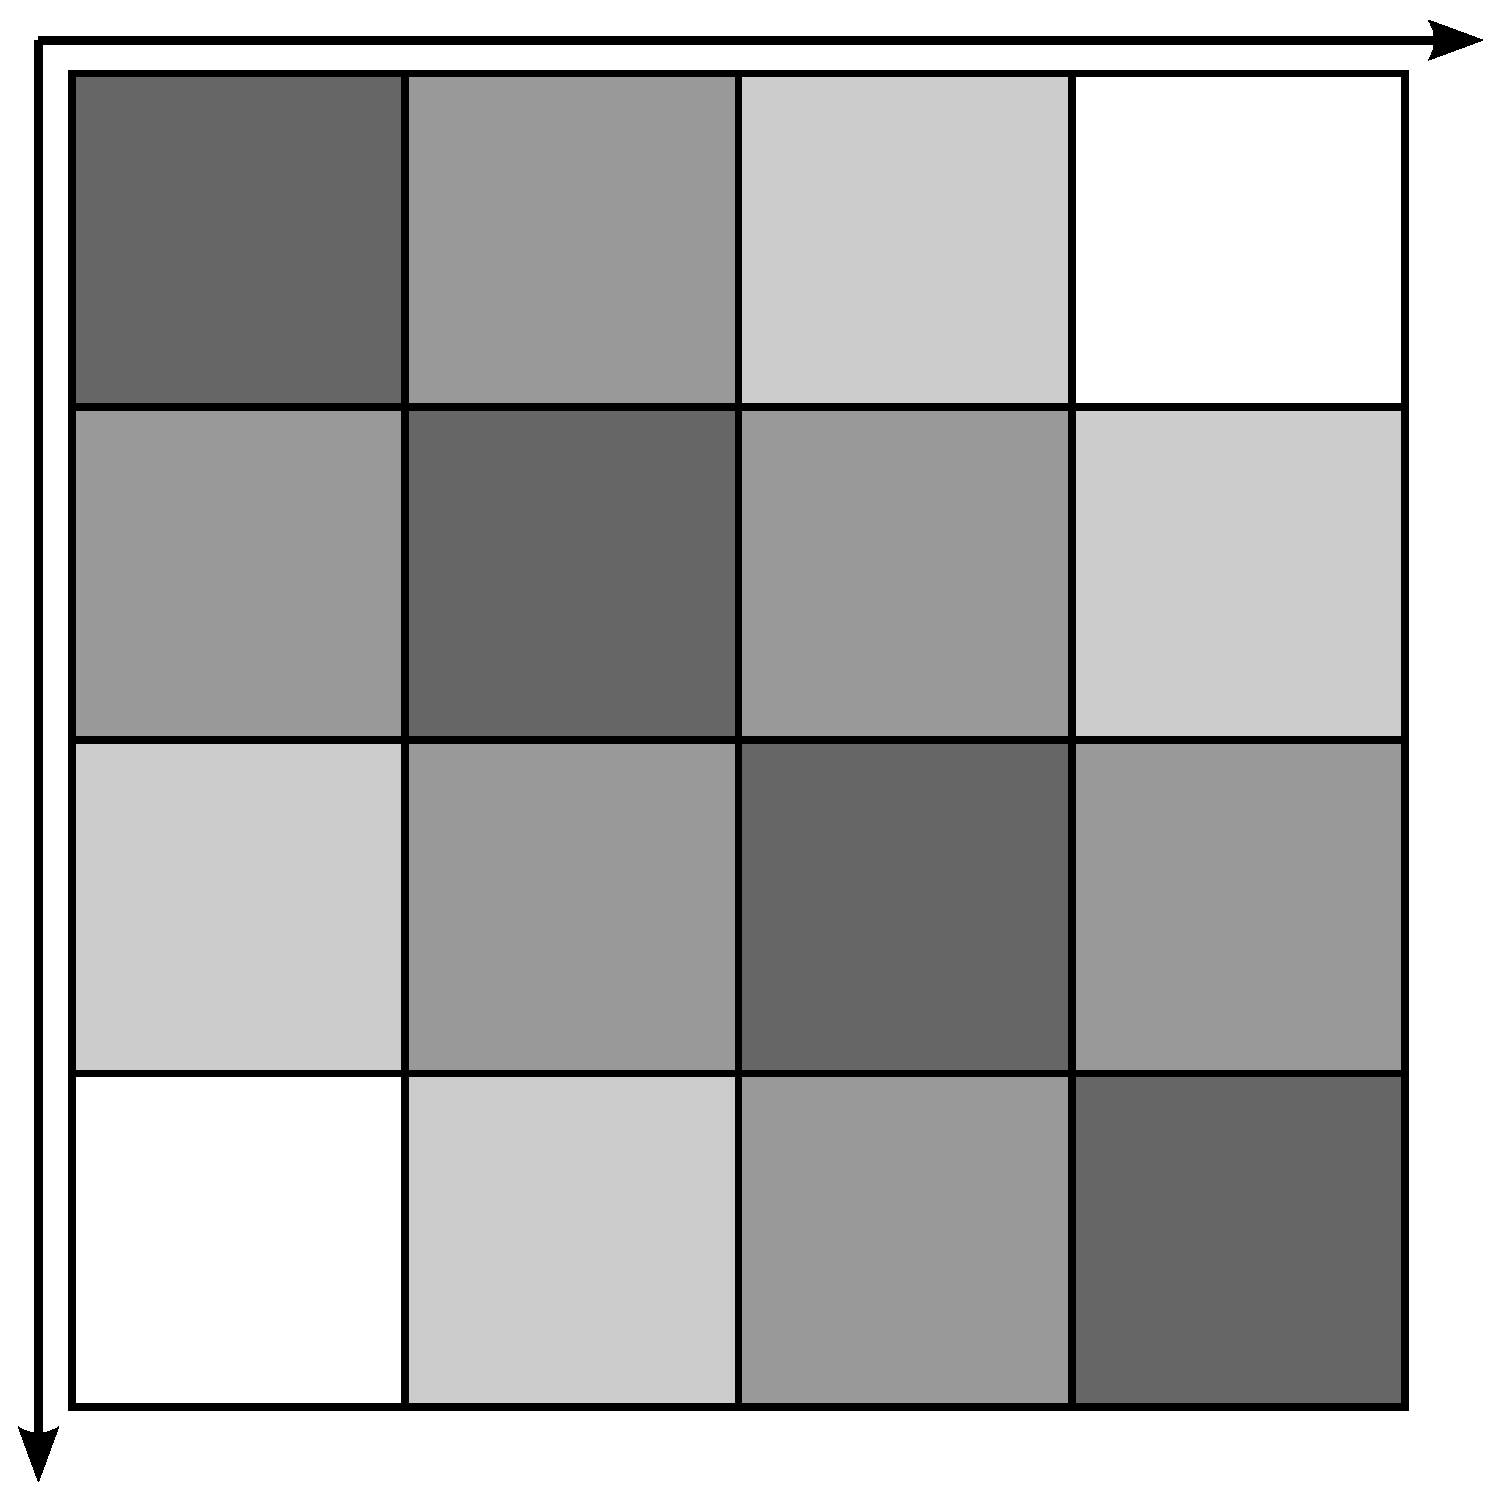
\includegraphics[width=0.46\unitlength]{thesis/talk/images/external/H_initial.eps}}
          \put(0.5400,0.0450){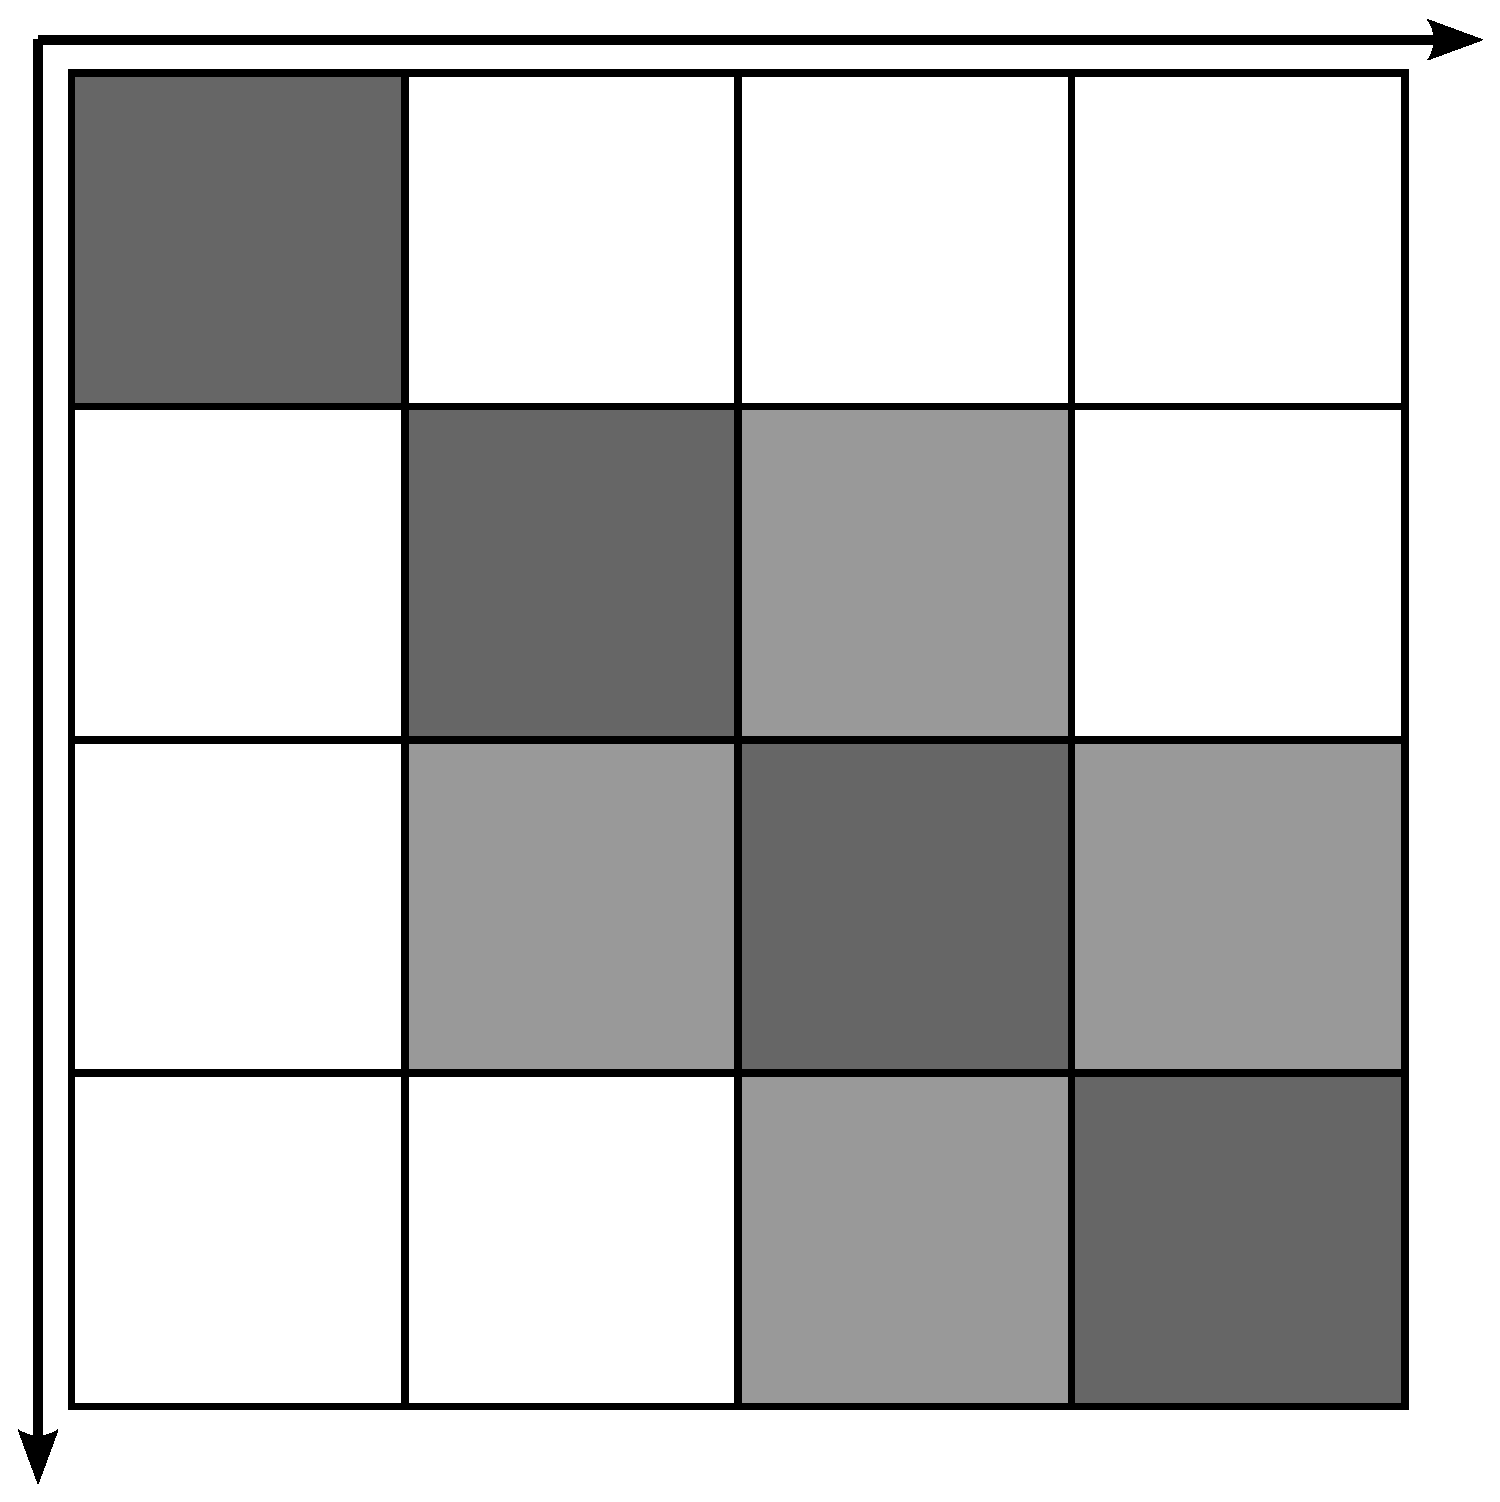
\includegraphics[width=0.46\unitlength]{thesis/talk/images/external/H_IMSRG_3ph_decoupling.eps}}
          \put(0.0100,0.0000){\parbox{0.5\unitlength}{\centering$\braket{i|H(s=0)|j}$}}
          \put(0.5200,0.0000){\parbox{0.5\unitlength}{\centering$\braket{i|H(s \rightarrow \infty)|j}$}}

          \put(0.0500,0.5100){\parbox{0.11\unitlength}{\centering\footnotesize0p0h}}
          \put(0.1600,0.5100){\parbox{0.11\unitlength}{\centering\footnotesize1p1h}}
          \put(0.2630,0.5100){\parbox{0.11\unitlength}{\centering\footnotesize2p2h}}
          \put(0.3650,0.5100){\parbox{0.11\unitlength}{\centering\footnotesize3p3h}}
          \put(0.5500,0.5100){\parbox{0.11\unitlength}{\centering\footnotesize0p0h}}
          \put(0.6600,0.5100){\parbox{0.11\unitlength}{\centering\footnotesize1p1h}}
          \put(0.7630,0.5100){\parbox{0.11\unitlength}{\centering\footnotesize2p2h}}
          \put(0.8650,0.5100){\parbox{0.11\unitlength}{\centering\footnotesize3p3h}}
          %
          \put(0.0070,0.4320){\parbox{0.11\unitlength}{\rotatebox{90}{\centering\footnotesize0p0h}}}
          \put(0.0070,0.3235){\parbox{0.11\unitlength}{\rotatebox{90}{\centering\footnotesize1p1h}}}
          \put(0.0070,0.2175){\parbox{0.11\unitlength}{\rotatebox{90}{\centering\footnotesize2p2h}}}
          \put(0.0070,0.1100){\parbox{0.11\unitlength}{\rotatebox{90}{\centering\footnotesize3p3h}}}

          \put(0.5100,0.4320){\parbox{0.11\unitlength}{\rotatebox{90}{\centering\footnotesize0p0h}}}
          \put(0.5100,0.3235){\parbox{0.11\unitlength}{\rotatebox{90}{\centering\footnotesize1p1h}}}
          \put(0.5100,0.2175){\parbox{0.11\unitlength}{\rotatebox{90}{\centering\footnotesize2p2h}}}
          \put(0.5100,0.1100){\parbox{0.11\unitlength}{\rotatebox{90}{\centering\footnotesize3p3h}}}
        \end{picture}
        \\
        {\tiny Hergert \textit{et al.}, Phys.~Rept.~\textbf{621}, 2016}
      \end{center}
    \end{column}
  \end{columns}
\end{frame}

\begin{frame}{Fundamental commutators}
  \vskip1.5em
  \begin{columns}
    \begin{column}{0.5\textwidth}
      ``Fundamental'': commutators are the  \\
      basic computational operation
      \begin{equation*}
        \left[A^{(K)}, B^{(L)} \right]= \sum_{M=|K-L|}^{K+L - 1} C^{(M)}
      \end{equation*}
      Schematic notation:
      \begin{equation*}
        [K, L] \rightarrow M
      \end{equation*}
      w/ computational cost $\mathcal{O}(N^{K+L+M})$ \\
      where $N$ is the size of the computational basis
    \end{column}
    \begin{column}{0.5\textwidth}
      \pause
      IMSRG(3) commutators:
      \begin{align*}
        \mathcal{O}(N^6):                                       &     &
        [1,3]                  \rightarrow 2                    & \,,
        [2,3] \rightarrow 1\,,
        [3,3] \rightarrow 0                                                                    \\
        \mathcal{O}(N^7):                                       &     &
        \textcolor{red}{[2,2]\rightarrow 3}                     & \,,
        [1,3] \rightarrow 3\,,
        [2,3] \rightarrow 2\,,                                                                 \\
                                                                &     & [3,3]  \rightarrow 1 & \\
        \mathcal{O}(N^8):                                       &     &
        [2,3]                  \rightarrow 3                    & \,,
        [3,3] \rightarrow 2                                                                    \\
        \mathcal{O}(N^9):                                       &     &
        \textcolor{blue}{[3,3]                   \rightarrow 3} &
      \end{align*}
      \vskip-1.0em
      \begin{itemize}
        \item $\textcolor{red}{[2, 2]\rightarrow 3}$ induces neglected three-body part in IMSRG(2)
        \item $\textcolor{blue}{[3, 3]\rightarrow 3}$ is most expensive
        \item Note: $\Lambda$-CCSD(T) is $\mathcal{O}(N^7)$
      \end{itemize}
    \end{column}
  \end{columns}
\end{frame}

\begin{frame}{IMSRG(3) computational challenges}
  \begin{columns}
    \begin{column}{0.55\textwidth}
      $O_{pqrstu}$:
      \begin{itemize}
        \item Rank-6 tensor with $\mathcal{O}(N^6)$ storage cost
        \item $\sim 30$ GB at $\emax=2$
      \end{itemize}
      \vskip1.0em
      $\sum_{abc} \genthree_{ijkabc} \hnothree_{abclmn}$:
      \begin{itemize}
        \item Huge matrix-matrix multiply
        \item $\mathcal{O}(10^{14})$ FLOPs at $\emax=2$
      \end{itemize}
      \vskip1.0em
      Challenging at $\emax=2$\\
      and larger model spaces out of reach
    \end{column}
    \begin{column}{0.35\textwidth}
      \pause
      Exploitable symmetries:
      \begin{itemize}
        \item Isospin conservation
        \item Parity conservation
        \item \textbf{Rotational invariance}
      \end{itemize}
    \end{column}
  \end{columns}
\end{frame}

\begin{frame}{Angular-momentum coupling for the IMSRG}
  \begin{itemize}
    \item Express everything in terms of eigenstates of $J_{z}$ and $J^2$
    \item Analytically simplify angular-momentum projection dependence
    \item Go from states $\ket{p}=\ket{\tilde{p}m_p}$ to ``reduced'' orbitals $\tilde{p}$
  \end{itemize}
  \pause
  \begin{center}
    \begin{tabular*}{0.9\textwidth}{l| l | l| l}
      & Basis & Uncoupled MEs & Coupled MEs \\
      \hline
      One-body & $\ket{\tilde{p} m_p}$ & $O_{pq}$ & $O^{j_{p}}_{\tilde{p}\tilde{q}}$ \\
      Two-body & $\ket{(\tilde{p} \tilde{q}) J_{pq} M_{pq}}$ & $O_{pqrs}$ & $O^{J_{pq}}_{\tilde{p}\tilde{q}\tilde{r}\tilde{s}}$ \\
      Three-body & $\ket{[(\tilde{p} \tilde{q}) J_{pq} \tilde{r}] J_{pqr} M_{pqr}}$ & $O_{pqrstu}$ & $O^{(J_{pqr}, J_{pq}, J_{rs})}_{\tilde{p}\tilde{q}\tilde{r}\tilde{s}\tilde{t}\tilde{u}}$
    \end{tabular*}
  \end{center}

  Automatic angular-momentum coupling of fundamental commutators \\
  performed using \texttt{amc} program {\tiny (Tichai \textit{et al.}, 2020)}

\end{frame}

\begin{frame}{${}^{4}\text{He}$ in IMSRG(2) {\tiny Hamiltonian details}}
  \vskip1.0em
  \begin{columns}
    \begin{column}{0.45\textwidth}
      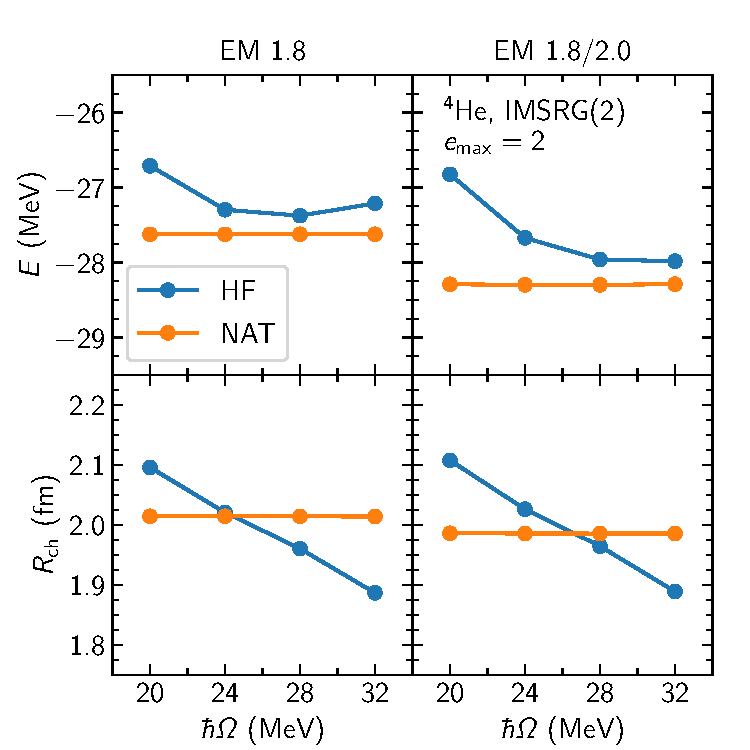
\includegraphics[width=\textwidth]{thesis/talk/images/he4_imsrg2_results.pdf}
    \end{column}
    \begin{column}{0.55\textwidth}
      \begin{equation*}
        H_{\text{int}} =
        T_{\text{int}} + V^{(2)} (+ V^{(3)})
      \end{equation*}
      NN-only case:
      \begin{itemize}
        \item \nthreelo{} EM potential with $\Lambda=450\mev$ \\
              SRG-evolved to $\lambda=1.8\invfm$
        \item ``EM 1.8''
      \end{itemize}
      \vskip0.5em
      NN+3N case (\textbf{NO2B}):
      \begin{itemize}
        \item 3N potential fit after SRG evolution \\
              to reproduce $E_{{}^{3}\text{H}}$ and $R_{{}^{4}\text{He}}$
        \item ``EM 1.8/2.0''
      \end{itemize}

    \end{column}
  \end{columns}
\end{frame}

\begin{frame}{${}^{4}\text{He}$ in IMSRG(2) {\tiny Basis details}}
  \vskip1.0em
  \begin{columns}
    \begin{column}{0.45\textwidth}
      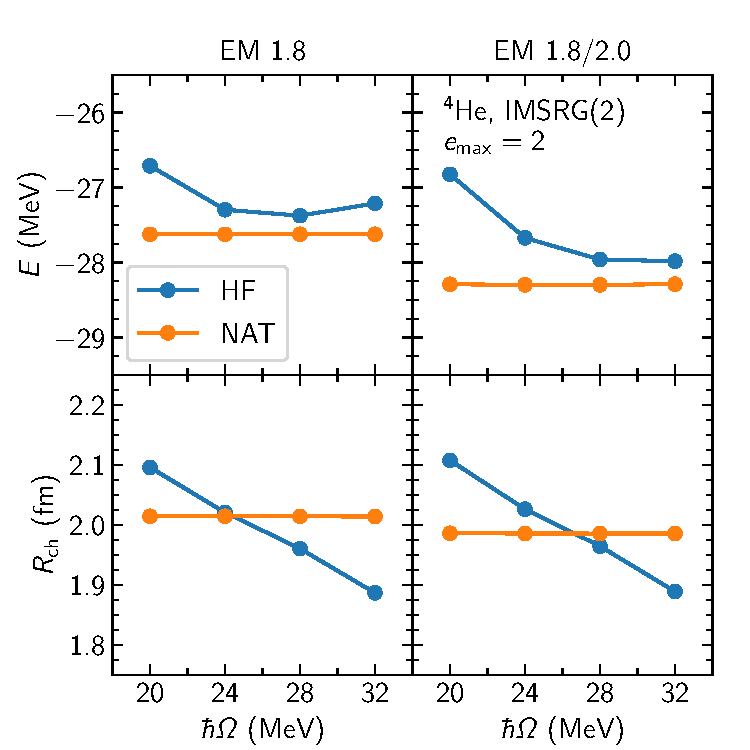
\includegraphics[width=\textwidth]{thesis/talk/images/he4_imsrg2_results.pdf}
    \end{column}
    \begin{column}{0.55\textwidth}
      $e=2n + l \leq \emax=2$ model space:
      \begin{itemize}
        \item 12 reduced orbitals $\tilde{p}$
        \item 6 two-body channels
        \item 132 three-body channels
      \end{itemize}
      \pause
      Hartree-Fock (HF) basis:
      \begin{itemize}
        \item Constructed in $\emax=2$
      \end{itemize}
      Natural orbitals (NAT) basis: {\tiny (Hoppe \textit{et al.}, 2020)}
      \begin{itemize}
        \item Eigenbasis of perturbatively-constructed density
        \item Constructed in $\emax=14$ ($E_{\text{3max}}=16$)
      \end{itemize}
    \end{column}
  \end{columns}
\end{frame}

\begin{frame}{${}^{4}\text{He}$ in IMSRG(2)}
  \vskip1.0em
  \begin{columns}
    \begin{column}{0.45\textwidth}
      \begin{overprint}
        \onslide<1>\centering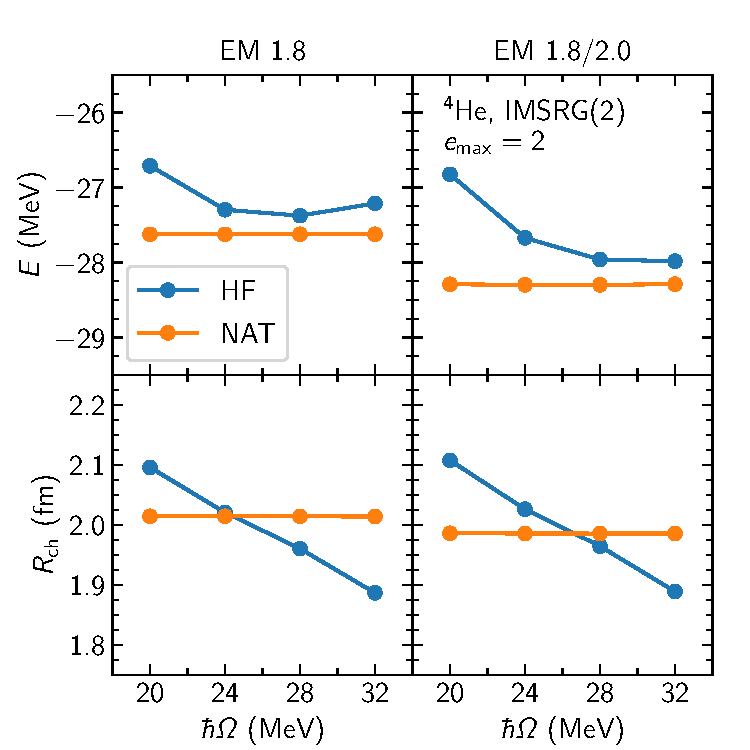
\includegraphics[width=\textwidth]{thesis/talk/images/he4_imsrg2_results.pdf}
        \onslide<2>\centering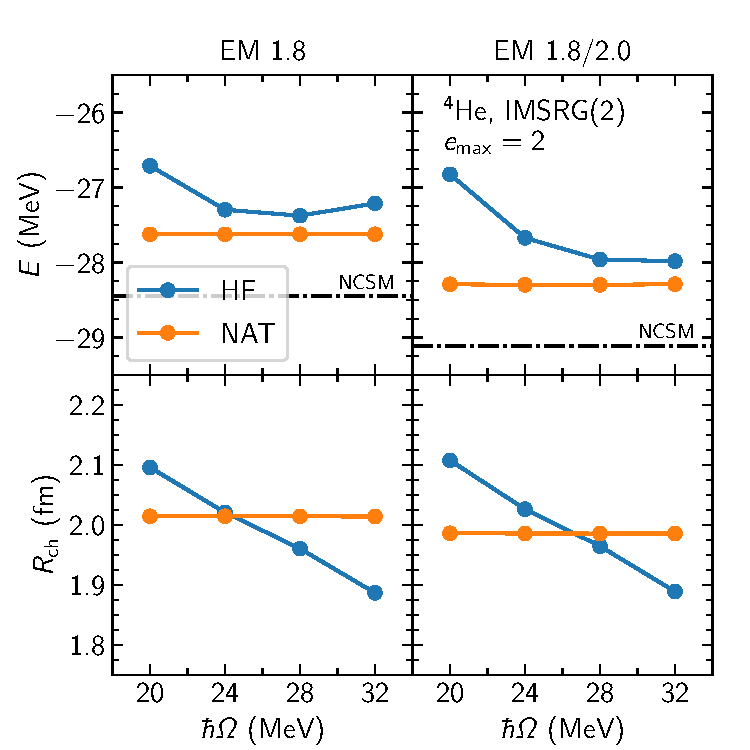
\includegraphics[width=\textwidth]{thesis/talk/images/he4_imsrg2_results_with_NCSM.pdf}
        \onslide<3->\centering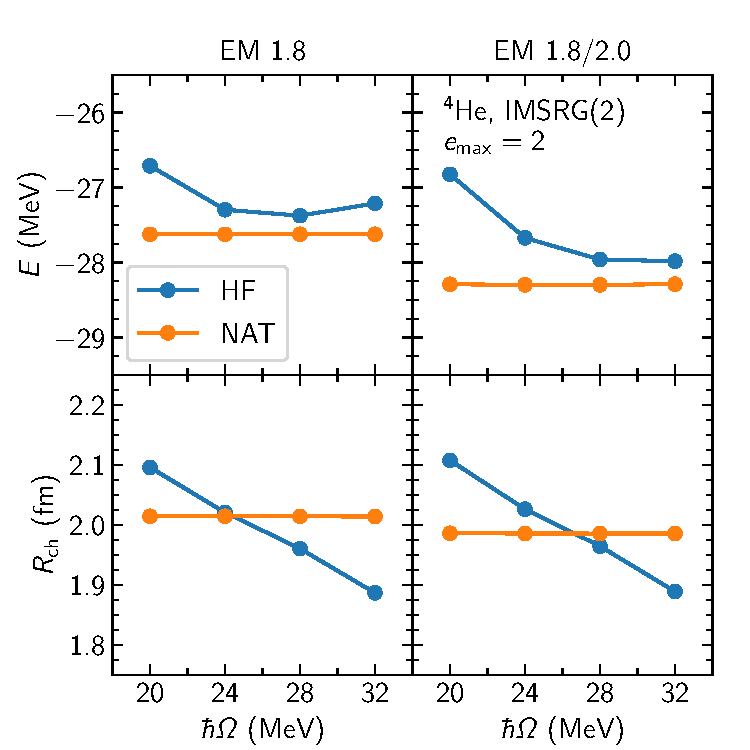
\includegraphics[width=\textwidth]{thesis/talk/images/he4_imsrg2_results.pdf}
      \end{overprint}
    \end{column}
    \begin{column}{0.55\textwidth}
      Disclaimer:\\
      \begin{itemize}
        \item $\emax=2$ results are not converged
        \item Cannot compare to experiment
        \item Ideal comparison would be to $\emax=2$ CI
      \end{itemize}
      \visible<4->{Trends:
        \begin{itemize}
          \item Inclusion of 3N forces gives slightly \\
                more binding energy \\
                and a slightly smaller charge radius
          \item NAT results are independent of $\hbar \Omega$
        \end{itemize}}
    \end{column}
  \end{columns}
\end{frame}

\begin{frame}{Approximate IMSRG(3) truncation schemes}
  \begin{columns}
    \begin{column}{0.4\textwidth}
      Idea:
      \begin{itemize}
        \item Start with IMSRG(2)
        \item Selectively add \\
              IMSRG(3) commutators
        \item Investigate which terms \\
              are most important
      \end{itemize}
      \pause
    \end{column}
    \begin{column}{0.6\textwidth}
      \begin{flalign*}
        \text{IMSRG(3)-A} &=
        \text{IMSRG(2)}
        + [2, 2] \rightarrow 3 \\
        & \quad
        + [2, 3] \rightarrow 2
        + [1, 3] \rightarrow 3
      \end{flalign*}
      \pause
      \vskip-4.0em
      \begin{flalign*}
        \text{IMSRG(3)-B} &=
        \text{IMSRG(3)-A}
        + [3, 3] \rightarrow 0 \\
        & \quad
        + [2, 3] \rightarrow 1
        + [1, 3] \rightarrow 2
      \end{flalign*}
      \pause
      \vskip-4.0em
      \begin{flalign*}
        \text{IMSRG(3)-C} &=
        \text{IMSRG(3)-B}
        + [3, 3] \rightarrow 1 \\
        &= \text{IMSRG(3)-$N^7$}
      \end{flalign*}
      \pause
      \vskip-4.0em
      \begin{flalign*}
        \text{IMSRG(3)-D} &=
        \text{IMSRG(3)-C}
        + [2, 3] \rightarrow 3
      \end{flalign*}
    \end{column}
  \end{columns}
\end{frame}

\begin{frame}{${}^{4}\text{He}$ in IMSRG(3)-$N^7$}
  \vskip1.0em
  \begin{columns}
    \begin{column}{0.45\textwidth}
      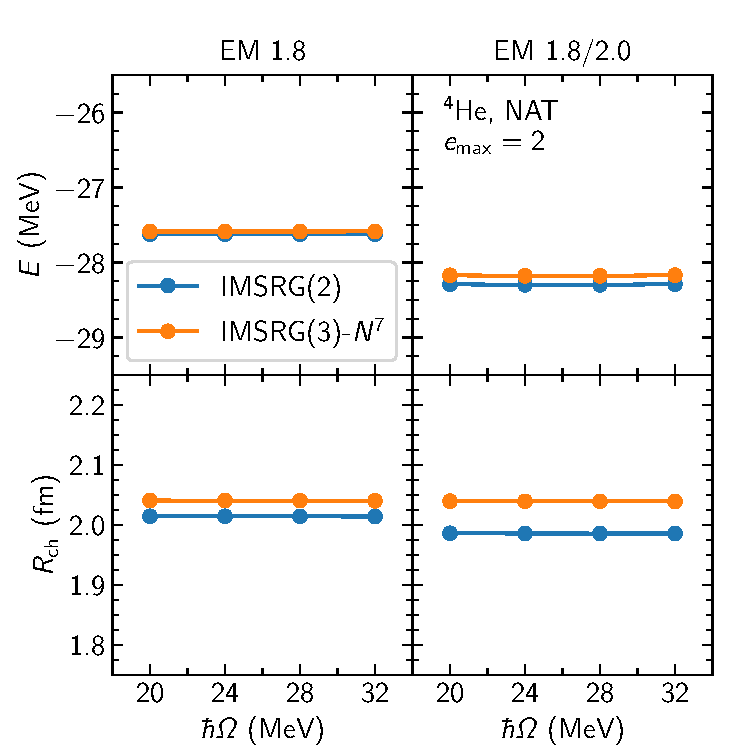
\includegraphics[width=\textwidth]{thesis/talk/images/he4_NAT_results.pdf}
    \end{column}
    \begin{column}{0.55\textwidth}
      \begin{itemize}
        \item Small effect on energies
              \begin{itemize}
                \item $\sim 40$ keV for NN-only
                \item $\sim 100$ keV for NN+3N
              \end{itemize}
        \item Larger effect on radii
              \begin{itemize}
                \item $\sim 0.025$ fm for NN-only
                \item $\sim 0.054$ fm for NN+3N
                \item Still in few percent range
              \end{itemize}
      \end{itemize}
    \end{column}
  \end{columns}
\end{frame}

\begin{frame}{${}^{4}\text{He}$ in IMSRG(3)-$N^7$}
  \vskip1.0em
  \begin{columns}
    \begin{column}{0.45\textwidth}
      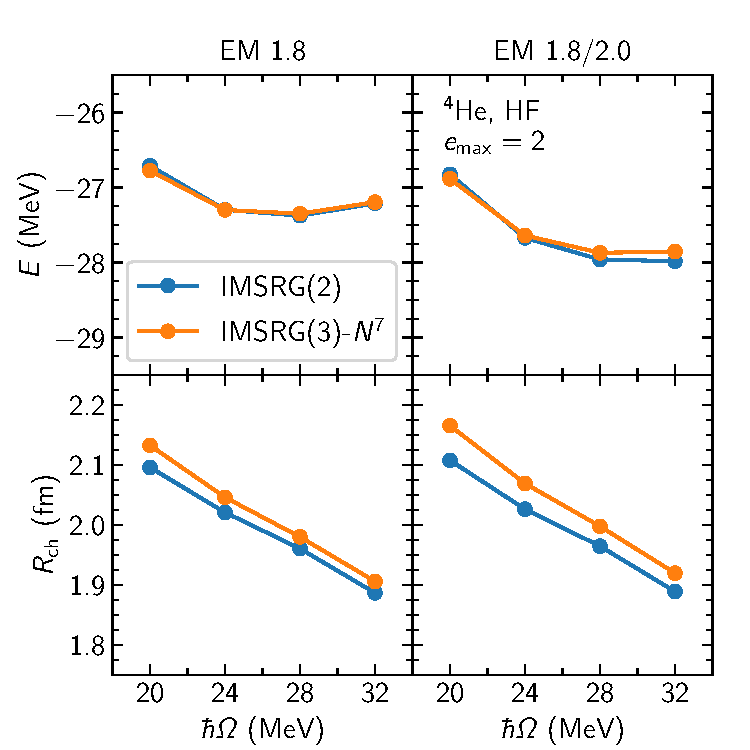
\includegraphics[width=\textwidth]{thesis/talk/images/he4_HF_results.pdf}
    \end{column}
    \begin{column}{0.55\textwidth}
      \begin{itemize}
        \item Same trends as NAT basis
        \item Freqency dependence seems slightly flatter in energies
        \item No similar behavior for radii
        \item Will be interesting to look at trends \\ in larger model spaces
      \end{itemize}
    \end{column}
  \end{columns}
\end{frame}

\begin{frame}{Truncation scheme investigation in ${}^{16}\text{O}$}
  \vskip1.0em
  \begin{columns}
    \begin{column}{0.45\textwidth}
      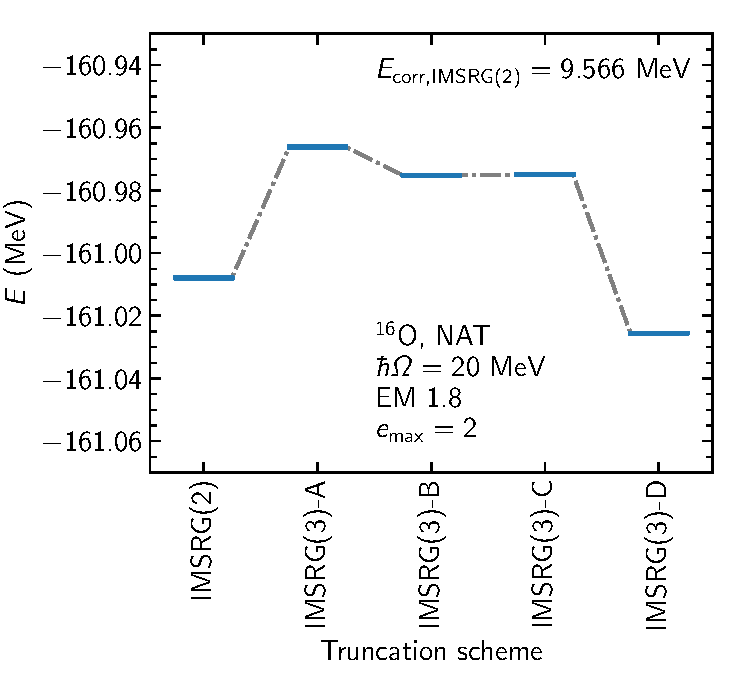
\includegraphics[width=\textwidth]{thesis/talk/images/term_by_term_o16_plot.pdf}
    \end{column}
    \begin{column}{0.55\textwidth}
      \begin{itemize}
        \item Overall, all corrections are small \\
              (sub-100 keV for 160 MeV binding energy)
        \item IMSRG(3)-A produces \\ a relatively large shift
        \item IMSRG(3)-B (with $\mathcal{O}(N^6)$ commutators) \\
              and IMSRG(3)-C produce very small shifts
        \item IMSRG(3)-D (first $\mathcal{O}(N^8)$ commutator) \\
              produces the largest shift
      \end{itemize}
    \end{column}
  \end{columns}
\end{frame}

\addtocounter{framenumber}{-1}

\begin{frame}{Truncation scheme investigation in ${}^{16}\text{O}$}
  \vskip1.0em
  \begin{columns}
    \begin{column}{0.45\textwidth}
      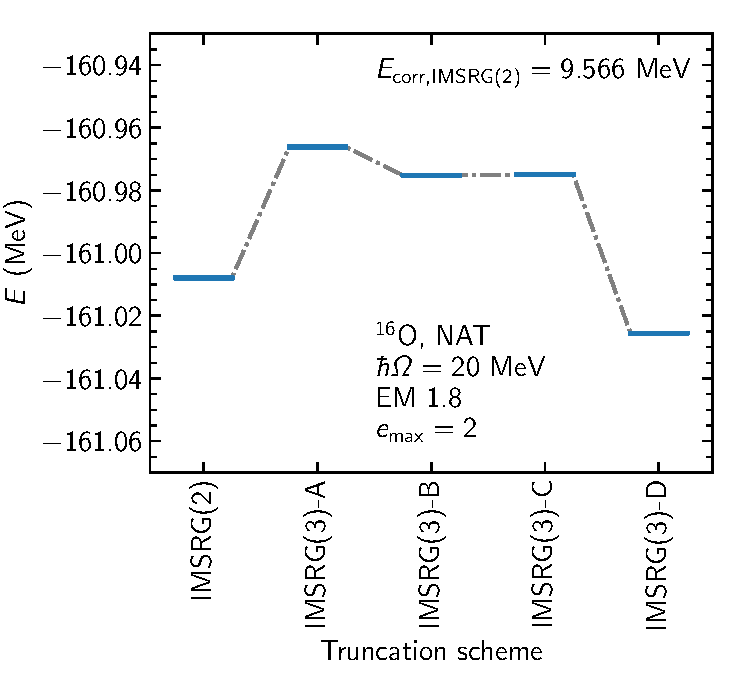
\includegraphics[width=\textwidth]{thesis/talk/images/term_by_term_o16_plot.pdf}
    \end{column}
    \begin{column}{0.55\textwidth}
      \begin{flalign*}
        \text{IMSRG(3)-A} &=
        \text{IMSRG(2)}
        + \textcolor{red}{[2, 2] \rightarrow 3} \\
        & \quad
        + \textcolor{red}{[2, 3] \rightarrow 2}
        + \textcolor{red}{[1, 3] \rightarrow 3}
      \end{flalign*}
      \vskip-2.5em
      \begin{flalign*}
        \text{IMSRG(3)-B} &=
        \text{IMSRG(3)-A}
        + [3, 3] \rightarrow 0 \\
        & \quad
        + [2, 3] \rightarrow 1
        + [1, 3] \rightarrow 2
      \end{flalign*}
      \vskip-2.5em
      \begin{flalign*}
        \text{IMSRG(3)-C} &=
        \text{IMSRG(3)-B}
        + [3, 3] \rightarrow 1 \\
        &= \text{IMSRG(3)-$N^7$}
      \end{flalign*}
      \vskip-2.5em
      \begin{flalign*}
        \text{IMSRG(3)-D} &=
        \text{IMSRG(3)-C}
        + \textcolor{blue}{[2, 3] \rightarrow 3}
      \end{flalign*}
    \end{column}
  \end{columns}
\end{frame}

\begin{frame}{Summary and outlook}
  \begin{columns}
    \begin{column}{0.5\textwidth}
      \begin{itemize}
        \item IMSRG(3)-$N^7$ gives corrections \\
              on the order of per mille for energies \\
              and few percent for radii
        \item Naive organization of fundamental commutators by cost was not successful
      \end{itemize}
    \end{column}
    \begin{column}{0.5\textwidth}
      \pause
      \begin{itemize}
        \item Extend the reach of the code to larger model spaces (goal: $\emax=6$)
        \item Use physical arguments to identify most important fundamental commutators
              for an approximate IMSRG(3) truncation
      \end{itemize}
    \end{column}
  \end{columns}
  \pause
  \begin{center}
    Thank you to my collaborators, Achim, Alex, Jan, Kai!
  \end{center}
  \pause
  \begin{center}
    \textbf{Thank you for your attention!}
  \end{center}
\end{frame}

\appendix
\backupbegin

\begin{frame}{Flow in ${}^{16}\text{O}$ - HF}
  \begin{columns}
    \begin{column}{0.5\textwidth}
      \begin{center}
        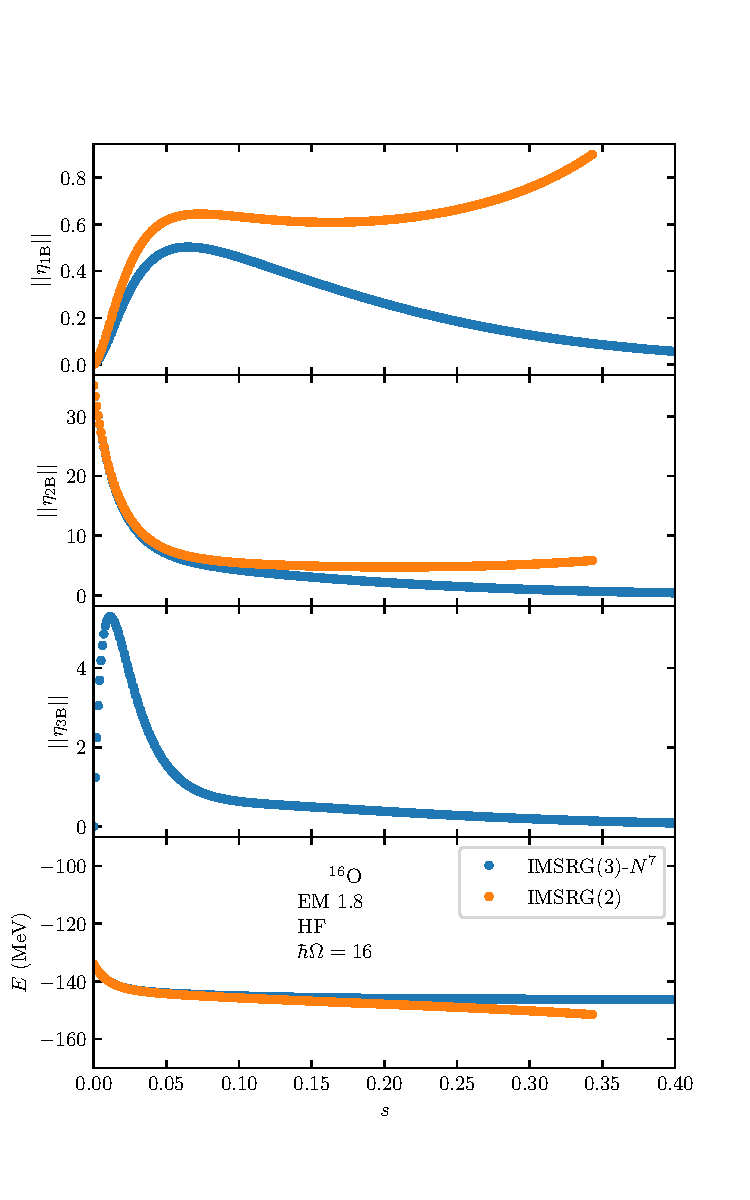
\includegraphics[trim=0 1.0cm 0 1.5cm, clip, width=0.7\textwidth]{thesis/talk/images/oxygen_flow_imsrg2_and_3_eta.pdf}
      \end{center}
    \end{column}
    \begin{column}{0.5\textwidth}
      \begin{center}
        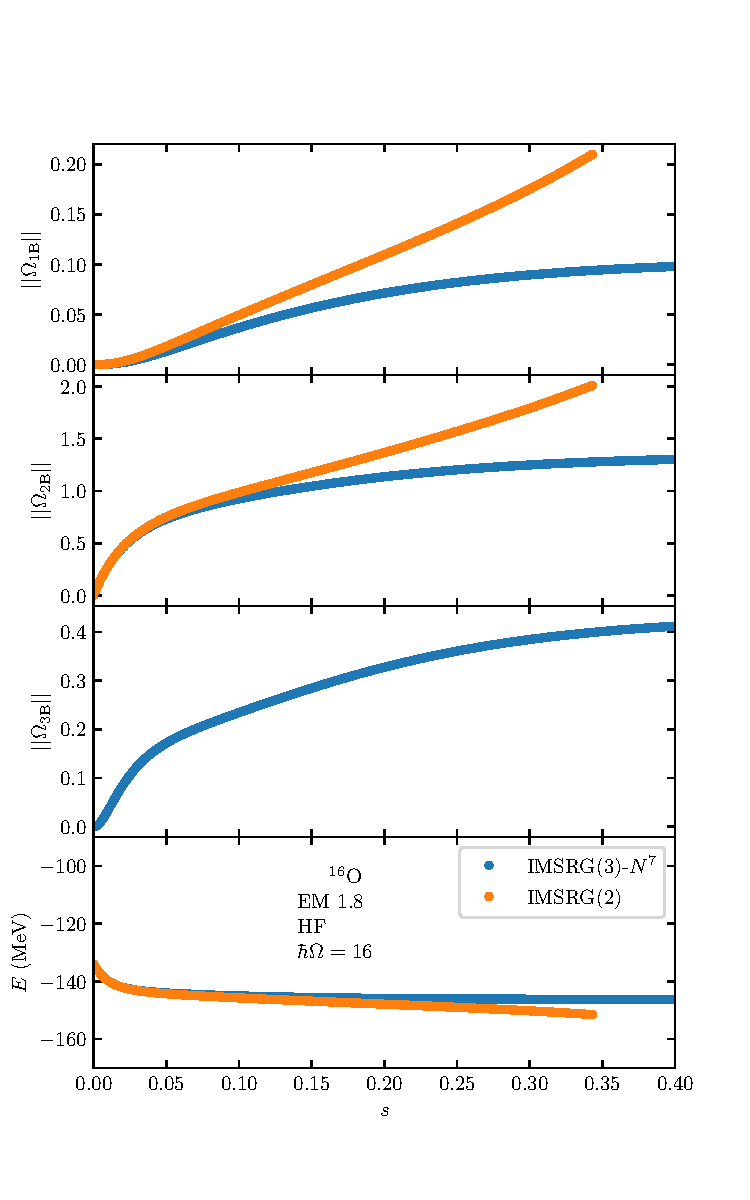
\includegraphics[trim=0 1.0cm 0 1.5cm, clip, width=0.7\textwidth]{thesis/talk/images/oxygen_flow_imsrg2_and_3_omega.pdf}
      \end{center}
    \end{column}

  \end{columns}
\end{frame}

\begin{frame}{Flow in ${}^{4}\text{He}$ - HF}
  \begin{columns}
    \begin{column}{0.5\textwidth}
      \begin{center}
        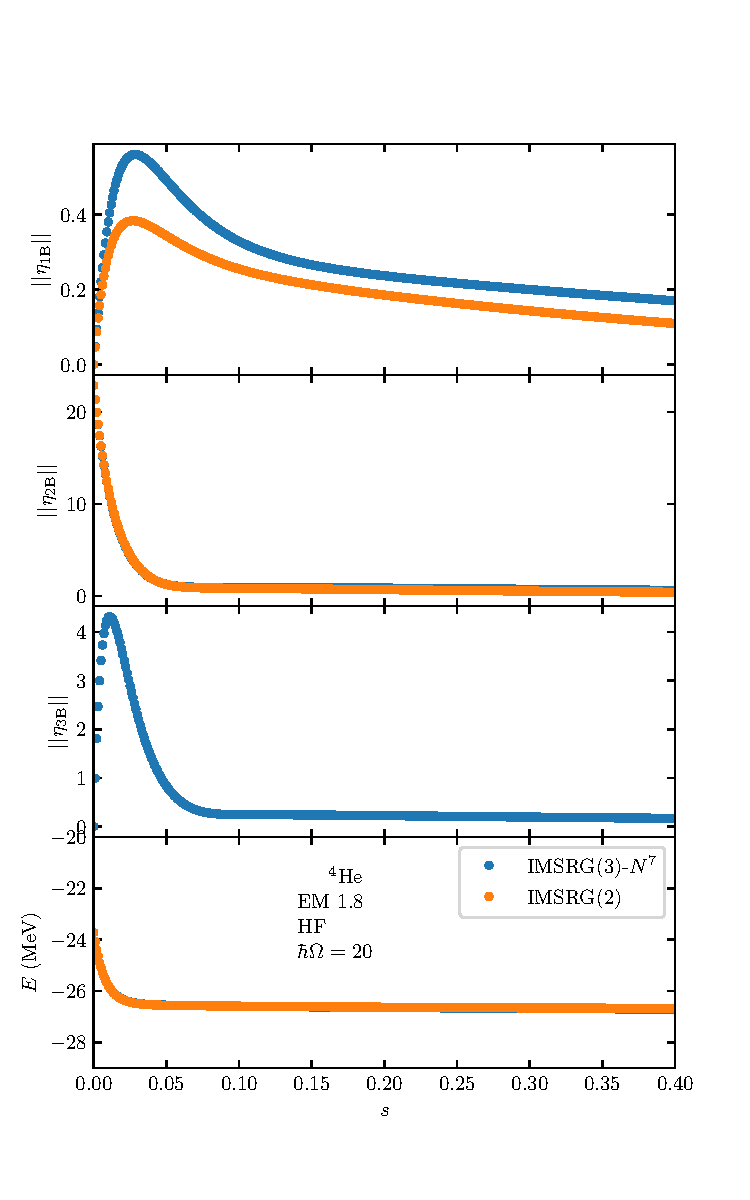
\includegraphics[trim=0 1.0cm 0 1.5cm, clip, width=0.7\textwidth]{thesis/talk/images/helium_flow_imsrg2_and_3_eta.pdf}
      \end{center}
    \end{column}
    \begin{column}{0.5\textwidth}
      \begin{center}
        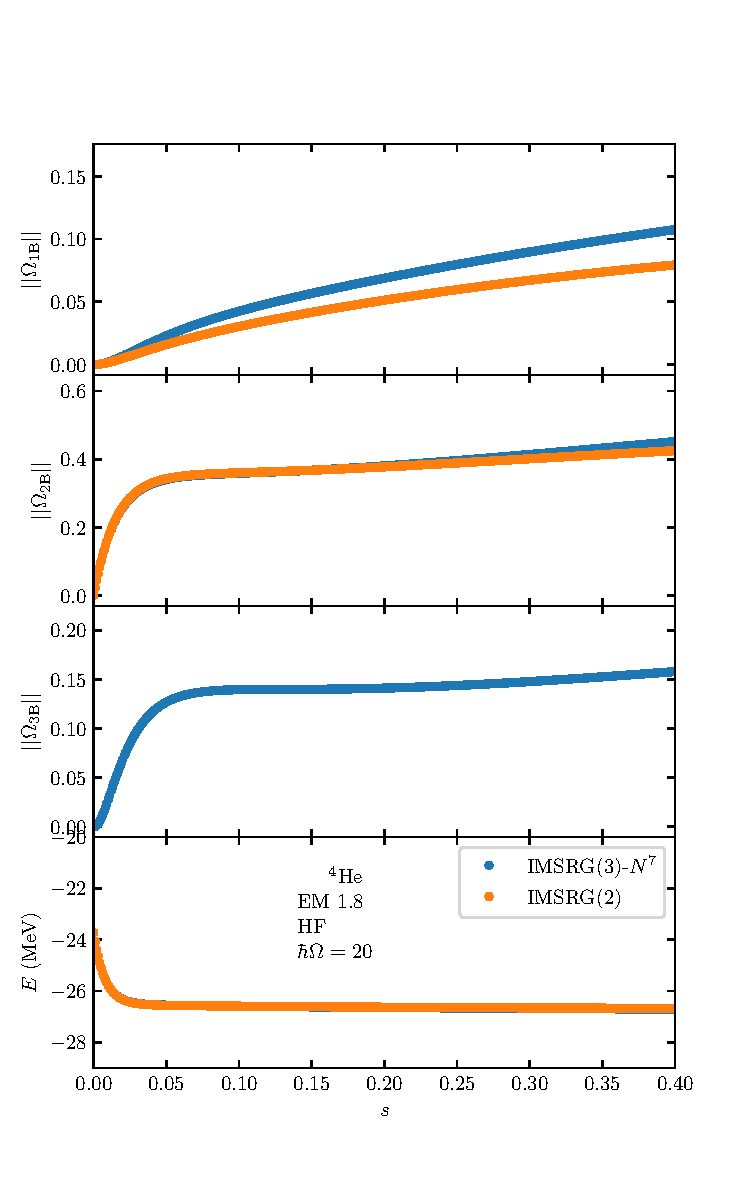
\includegraphics[trim=0 1.0cm 0 1.5cm, clip, width=0.7\textwidth]{thesis/talk/images/helium_flow_imsrg2_and_3_omega.pdf}
      \end{center}
    \end{column}

  \end{columns}
\end{frame}

\backupend


\end{document}
